\documentclass{standalone}
\usepackage{tikz}
\usetikzlibrary{patterns, positioning}


\begin{document}
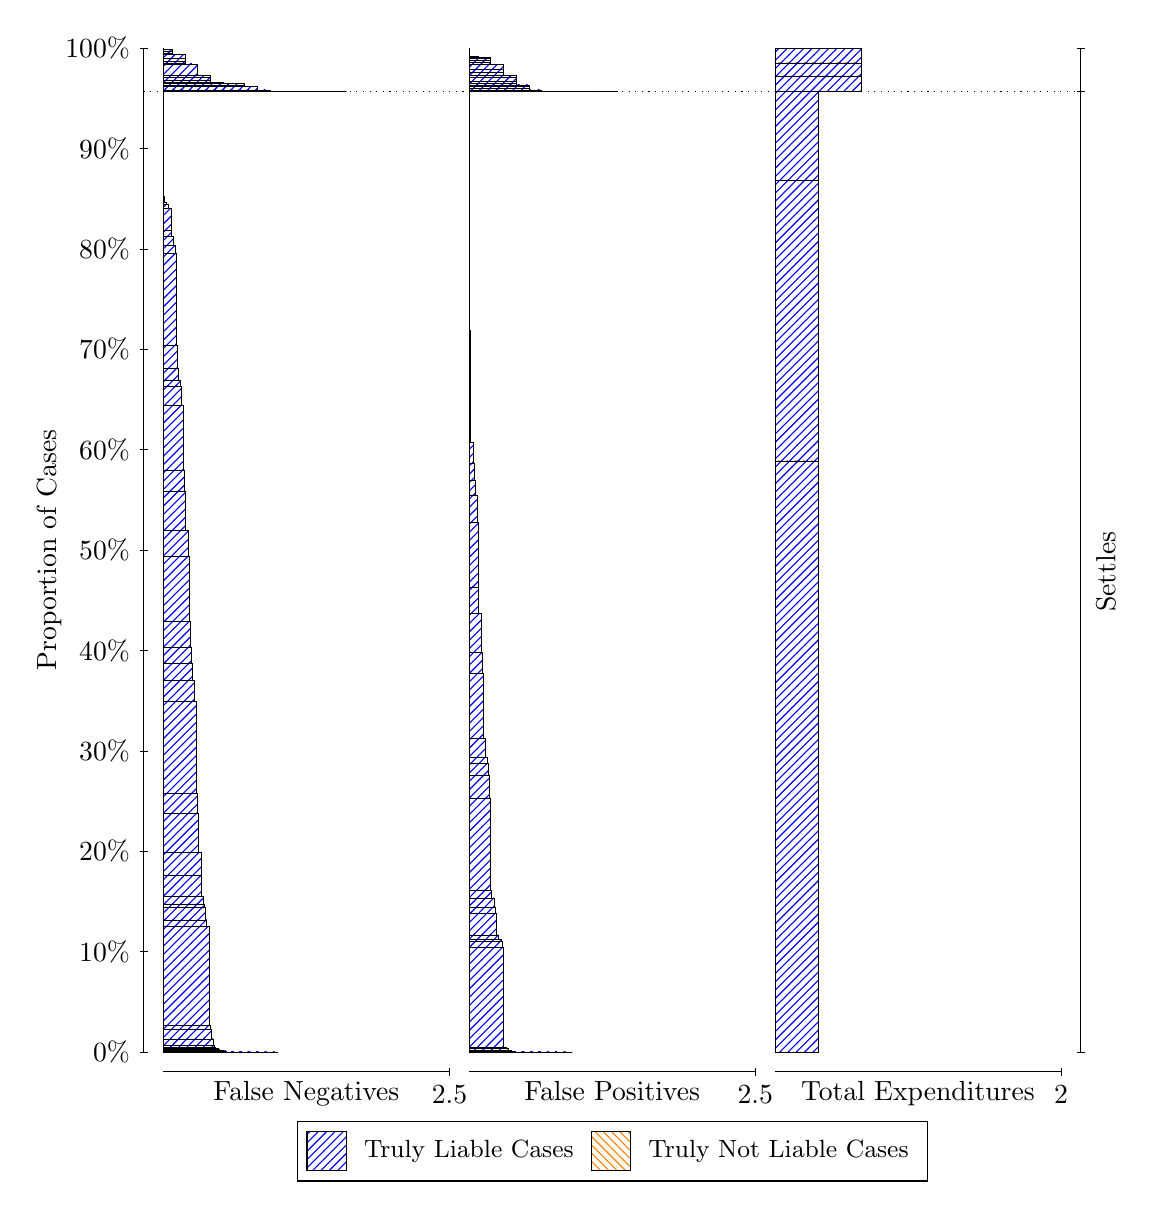
\begin{tikzpicture}
\draw[black, very thin] (1.5,1.75) -- (1.5,14.5);
\node[rotate=90, text=black, anchor=center] at (0.3, 8.125) {Proportion of Cases};
\draw[black, very thin] (1.45,1.75) -- (1.55,1.75);
\node[text=black, anchor=east] at (1.45, 1.75) {0\%};
\draw[black, very thin] (1.45,3.025) -- (1.55,3.025);
\node[text=black, anchor=east] at (1.45, 3.025) {10\%};
\draw[black, very thin] (1.45,4.3) -- (1.55,4.3);
\node[text=black, anchor=east] at (1.45, 4.3) {20\%};
\draw[black, very thin] (1.45,5.575) -- (1.55,5.575);
\node[text=black, anchor=east] at (1.45, 5.575) {30\%};
\draw[black, very thin] (1.45,6.85) -- (1.55,6.85);
\node[text=black, anchor=east] at (1.45, 6.85) {40\%};
\draw[black, very thin] (1.45,8.125) -- (1.55,8.125);
\node[text=black, anchor=east] at (1.45, 8.125) {50\%};
\draw[black, very thin] (1.45,9.4) -- (1.55,9.4);
\node[text=black, anchor=east] at (1.45, 9.4) {60\%};
\draw[black, very thin] (1.45,10.675) -- (1.55,10.675);
\node[text=black, anchor=east] at (1.45, 10.675) {70\%};
\draw[black, very thin] (1.45,11.95) -- (1.55,11.95);
\node[text=black, anchor=east] at (1.45, 11.95) {80\%};
\draw[black, very thin] (1.45,13.225) -- (1.55,13.225);
\node[text=black, anchor=east] at (1.45, 13.225) {90\%};
\draw[black, very thin] (1.45,14.5) -- (1.55,14.5);
\node[text=black, anchor=east] at (1.45, 14.5) {100\%};

\draw[black, very thin] (13.4,1.75) -- (13.4,14.5);
\draw[black, very thin] (13.35,1.75) -- (13.45,1.75);
\node[anchor=west] at (13.35, 1.75) {};
\draw[black, very thin] (13.35,13.947) -- (13.45,13.947);
\node[anchor=west] at (13.35, 13.947) {};
\draw[black, very thin] (13.35,14.5) -- (13.45,14.5);
\node[anchor=west] at (13.35, 14.5) {};

\draw[black, very thin, pattern color=blue, pattern=north east lines] (1.75,1.75) rectangle (3.2033,1.75);
\draw[black, very thin, pattern color=blue, pattern=north east lines] (1.75,1.75) rectangle (3.058,1.75);
\draw[black, very thin, pattern color=blue, pattern=north east lines] (1.75,1.75) rectangle (3.0419,1.75);
\draw[black, very thin, pattern color=blue, pattern=north east lines] (1.75,1.75) rectangle (2.9853,1.75);
\draw[black, very thin, pattern color=blue, pattern=north east lines] (1.75,1.75) rectangle (2.9127,1.75);
\draw[black, very thin, pattern color=blue, pattern=north east lines] (1.75,1.75) rectangle (2.8965,1.75);
\draw[black, very thin, pattern color=blue, pattern=north east lines] (1.75,1.75) rectangle (2.8804,1.75);
\draw[black, very thin, pattern color=blue, pattern=north east lines] (1.75,1.75) rectangle (2.84,1.75);
\draw[black, very thin, pattern color=blue, pattern=north east lines] (1.75,1.75) rectangle (2.8239,1.75);
\draw[black, very thin, pattern color=blue, pattern=north east lines] (1.75,1.75) rectangle (2.7673,1.75);
\draw[black, very thin, pattern color=blue, pattern=north east lines] (1.75,1.75) rectangle (2.7512,1.75);
\draw[black, very thin, pattern color=blue, pattern=north east lines] (1.75,1.75) rectangle (2.735,1.75);
\draw[black, very thin, pattern color=blue, pattern=north east lines] (1.75,1.75) rectangle (2.7189,1.75);
\draw[black, very thin, pattern color=blue, pattern=north east lines] (1.75,1.75) rectangle (2.6785,1.7501);
\draw[black, very thin, pattern color=blue, pattern=north east lines] (1.75,1.7501) rectangle (2.6624,1.7501);
\draw[black, very thin, pattern color=blue, pattern=north east lines] (1.75,1.7501) rectangle (2.622,1.7505);
\draw[black, very thin, pattern color=blue, pattern=north east lines] (1.75,1.7505) rectangle (2.6059,1.7511);
\draw[black, very thin, pattern color=blue, pattern=north east lines] (1.75,1.7511) rectangle (2.5897,1.7511);
\draw[black, very thin, pattern color=blue, pattern=north east lines] (1.75,1.7511) rectangle (2.5736,1.7511);
\draw[black, very thin, pattern color=blue, pattern=north east lines] (1.75,1.7511) rectangle (2.5574,1.7517);
\draw[black, very thin, pattern color=blue, pattern=north east lines] (1.75,1.7517) rectangle (2.5493,1.7627);
\draw[black, very thin, pattern color=blue, pattern=north east lines] (1.75,1.7627) rectangle (2.517,1.7684);
\draw[black, very thin, pattern color=blue, pattern=north east lines] (1.75,1.7684) rectangle (2.5009,1.7708);
\draw[black, very thin, pattern color=blue, pattern=north east lines] (1.75,1.7708) rectangle (2.4605,1.7792);
\draw[black, very thin, pattern color=blue, pattern=north east lines] (1.75,1.7792) rectangle (2.4444,1.8003);
\draw[black, very thin, pattern color=blue, pattern=north east lines] (1.75,1.8003) rectangle (2.4282,1.8026);
\draw[black, very thin, pattern color=blue, pattern=north east lines] (1.75,1.8026) rectangle (2.4121,1.8077);
\draw[black, very thin, pattern color=blue, pattern=north east lines] (1.75,1.8077) rectangle (2.3959,1.834);
\draw[black, very thin, pattern color=blue, pattern=north east lines] (1.75,1.834) rectangle (2.3879,1.9163);
\draw[black, very thin, pattern color=blue, pattern=north east lines] (1.75,1.9163) rectangle (2.3556,2.0329);
\draw[black, very thin, pattern color=blue, pattern=north east lines] (1.75,2.0329) rectangle (2.3394,2.0861);
\draw[black, very thin, pattern color=blue, pattern=north east lines] (1.75,2.0861) rectangle (2.3313,3.3492);
\draw[black, very thin, pattern color=blue, pattern=north east lines] (1.75,3.3492) rectangle (2.299,3.4289);
\draw[black, very thin, pattern color=blue, pattern=north east lines] (1.75,3.4289) rectangle (2.2829,3.582);
\draw[black, very thin, pattern color=blue, pattern=north east lines] (1.75,3.582) rectangle (2.2667,3.6303);
\draw[black, very thin, pattern color=blue, pattern=north east lines] (1.75,3.6303) rectangle (2.2506,3.7254);
\draw[black, very thin, pattern color=blue, pattern=north east lines] (1.75,3.7254) rectangle (2.2344,3.9972);
\draw[black, very thin, pattern color=blue, pattern=north east lines] (1.75,3.9972) rectangle (2.2264,4.2865);
\draw[black, very thin, pattern color=blue, pattern=north east lines] (1.75,4.2865) rectangle (2.1941,4.784);
\draw[black, very thin, pattern color=blue, pattern=north east lines] (1.75,4.784) rectangle (2.1779,5.0297);
\draw[black, very thin, pattern color=blue, pattern=north east lines] (1.75,5.0297) rectangle (2.1699,6.2056);
\draw[black, very thin, pattern color=blue, pattern=north east lines] (1.75,6.2056) rectangle (2.1376,6.4722);
\draw[black, very thin, pattern color=blue, pattern=north east lines] (1.75,6.4722) rectangle (2.1214,6.691);
\draw[black, very thin, pattern color=blue, pattern=north east lines] (1.75,6.691) rectangle (2.1053,6.8835);
\draw[black, very thin, pattern color=blue, pattern=north east lines] (1.75,6.8835) rectangle (2.0891,7.2212);
\draw[black, very thin, pattern color=blue, pattern=north east lines] (1.75,7.2212) rectangle (2.073,8.0412);
\draw[black, very thin, pattern color=blue, pattern=north east lines] (1.75,8.0412) rectangle (2.0649,8.3789);
\draw[black, very thin, pattern color=blue, pattern=north east lines] (1.75,8.3789) rectangle (2.0326,8.8763);
\draw[black, very thin, pattern color=blue, pattern=north east lines] (1.75,8.8763) rectangle (2.0164,9.1429);
\draw[black, very thin, pattern color=blue, pattern=north east lines] (1.75,9.1429) rectangle (2.0084,9.963);
\draw[black, very thin, pattern color=blue, pattern=north east lines] (1.75,9.963) rectangle (1.9761,10.209);
\draw[black, very thin, pattern color=blue, pattern=north east lines] (1.75,10.209) rectangle (1.9599,10.283);
\draw[black, very thin, pattern color=blue, pattern=north east lines] (1.75,10.283) rectangle (1.9438,10.431);
\draw[black, very thin, pattern color=blue, pattern=north east lines] (1.75,10.431) rectangle (1.9276,10.72);
\draw[black, very thin, pattern color=blue, pattern=north east lines] (1.75,10.72) rectangle (1.9115,11.896);
\draw[black, very thin, pattern color=blue, pattern=north east lines] (1.75,11.896) rectangle (1.9034,11.991);
\draw[black, very thin, pattern color=blue, pattern=north east lines] (1.75,11.991) rectangle (1.8711,12.108);
\draw[black, very thin, pattern color=blue, pattern=north east lines] (1.75,12.108) rectangle (1.855,12.187);
\draw[black, very thin, pattern color=blue, pattern=north east lines] (1.75,12.187) rectangle (1.8469,12.459);
\draw[black, very thin, pattern color=blue, pattern=north east lines] (1.75,12.459) rectangle (1.8146,12.512);
\draw[black, very thin, pattern color=blue, pattern=north east lines] (1.75,12.512) rectangle (1.7984,12.52);
\draw[black, very thin, pattern color=blue, pattern=north east lines] (1.75,12.52) rectangle (1.7823,12.541);
\draw[black, very thin, pattern color=blue, pattern=north east lines] (1.75,12.541) rectangle (1.7661,12.623);
\draw[black, very thin, pattern color=orange, pattern=north west lines] (1.75,12.623) rectangle (1.75,12.623);
\draw[black, very thin, pattern color=blue, pattern=north east lines] (1.75,12.623) rectangle (1.75,13.947);
\draw[black, very thin, pattern color=blue, pattern=north east lines] (1.75,13.947) rectangle (4.0753,13.947);
\draw[black, very thin, pattern color=blue, pattern=north east lines] (1.75,13.947) rectangle (3.9139,13.947);
\draw[black, very thin, pattern color=blue, pattern=north east lines] (1.75,13.947) rectangle (3.7524,13.947);
\draw[black, very thin, pattern color=blue, pattern=north east lines] (1.75,13.947) rectangle (3.5909,13.947);
\draw[black, very thin, pattern color=blue, pattern=north east lines] (1.75,13.947) rectangle (3.4294,13.948);
\draw[black, very thin, pattern color=blue, pattern=north east lines] (1.75,13.948) rectangle (3.3164,13.948);
\draw[black, very thin, pattern color=blue, pattern=north east lines] (1.75,13.948) rectangle (3.2679,13.949);
\draw[black, very thin, pattern color=blue, pattern=north east lines] (1.75,13.949) rectangle (3.2679,13.951);
\draw[black, very thin, pattern color=blue, pattern=north east lines] (1.75,13.951) rectangle (3.1549,13.951);
\draw[black, very thin, pattern color=blue, pattern=north east lines] (1.75,13.951) rectangle (3.1549,13.951);
\draw[black, very thin, pattern color=blue, pattern=north east lines] (1.75,13.951) rectangle (3.1064,13.969);
\draw[black, very thin, pattern color=blue, pattern=north east lines] (1.75,13.969) rectangle (2.9934,13.969);
\draw[black, very thin, pattern color=blue, pattern=north east lines] (1.75,13.969) rectangle (2.9934,13.969);
\draw[black, very thin, pattern color=blue, pattern=north east lines] (1.75,13.969) rectangle (2.945,14.014);
\draw[black, very thin, pattern color=blue, pattern=north east lines] (1.75,14.014) rectangle (2.8319,14.014);
\draw[black, very thin, pattern color=blue, pattern=north east lines] (1.75,14.014) rectangle (2.7835,14.026);
\draw[black, very thin, pattern color=blue, pattern=north east lines] (1.75,14.026) rectangle (2.7835,14.047);
\draw[black, very thin, pattern color=blue, pattern=north east lines] (1.75,14.047) rectangle (2.6704,14.047);
\draw[black, very thin, pattern color=blue, pattern=north east lines] (1.75,14.047) rectangle (2.622,14.052);
\draw[black, very thin, pattern color=blue, pattern=north east lines] (1.75,14.052) rectangle (2.509,14.053);
\draw[black, very thin, pattern color=blue, pattern=north east lines] (1.75,14.053) rectangle (2.509,14.068);
\draw[black, very thin, pattern color=blue, pattern=north east lines] (1.75,14.068) rectangle (2.4605,14.068);
\draw[black, very thin, pattern color=blue, pattern=north east lines] (1.75,14.068) rectangle (2.3475,14.068);
\draw[black, very thin, pattern color=blue, pattern=north east lines] (1.75,14.068) rectangle (2.3475,14.088);
\draw[black, very thin, pattern color=blue, pattern=north east lines] (1.75,14.088) rectangle (2.3475,14.126);
\draw[black, very thin, pattern color=blue, pattern=north east lines] (1.75,14.126) rectangle (2.3475,14.155);
\draw[black, very thin, pattern color=blue, pattern=north east lines] (1.75,14.155) rectangle (2.299,14.155);
\draw[black, very thin, pattern color=blue, pattern=north east lines] (1.75,14.155) rectangle (2.186,14.157);
\draw[black, very thin, pattern color=blue, pattern=north east lines] (1.75,14.157) rectangle (2.186,14.298);
\draw[black, very thin, pattern color=blue, pattern=north east lines] (1.75,14.298) rectangle (2.1376,14.298);
\draw[black, very thin, pattern color=blue, pattern=north east lines] (1.75,14.298) rectangle (2.0245,14.311);
\draw[black, very thin, pattern color=blue, pattern=north east lines] (1.75,14.311) rectangle (2.0245,14.328);
\draw[black, very thin, pattern color=blue, pattern=north east lines] (1.75,14.328) rectangle (2.0245,14.372);
\draw[black, very thin, pattern color=blue, pattern=north east lines] (1.75,14.372) rectangle (2.0245,14.416);
\draw[black, very thin, pattern color=blue, pattern=north east lines] (1.75,14.416) rectangle (1.9761,14.416);
\draw[black, very thin, pattern color=blue, pattern=north east lines] (1.75,14.416) rectangle (1.863,14.437);
\draw[black, very thin, pattern color=blue, pattern=north east lines] (1.75,14.437) rectangle (1.863,14.464);
\draw[black, very thin, pattern color=blue, pattern=north east lines] (1.75,14.464) rectangle (1.863,14.478);
\draw[black, very thin, pattern color=orange, pattern=north west lines] (1.75,14.478) rectangle (1.75,14.478);
\draw[black, very thin, pattern color=blue, pattern=north east lines] (1.75,14.478) rectangle (1.75,14.5);
\draw[black, very thin, pattern color=orange, pattern=north west lines] (5.6333,1.75) rectangle (6.9413,1.75);
\draw[black, very thin, pattern color=blue, pattern=north east lines] (5.6333,1.75) rectangle (6.9413,1.75);
\draw[black, very thin, pattern color=blue, pattern=north east lines] (5.6333,1.75) rectangle (6.7799,1.75);
\draw[black, very thin, pattern color=orange, pattern=north west lines] (5.6333,1.75) rectangle (6.7233,1.75);
\draw[black, very thin, pattern color=blue, pattern=north east lines] (5.6333,1.75) rectangle (6.7233,1.75);
\draw[black, very thin, pattern color=orange, pattern=north west lines] (5.6333,1.75) rectangle (6.6507,1.75);
\draw[black, very thin, pattern color=blue, pattern=north east lines] (5.6333,1.75) rectangle (6.6507,1.75);
\draw[black, very thin, pattern color=blue, pattern=north east lines] (5.6333,1.75) rectangle (6.6184,1.75);
\draw[black, very thin, pattern color=blue, pattern=north east lines] (5.6333,1.75) rectangle (6.5619,1.75);
\draw[black, very thin, pattern color=orange, pattern=north west lines] (5.6333,1.75) rectangle (6.5053,1.75);
\draw[black, very thin, pattern color=blue, pattern=north east lines] (5.6333,1.75) rectangle (6.5053,1.75);
\draw[black, very thin, pattern color=blue, pattern=north east lines] (5.6333,1.75) rectangle (6.4892,1.75);
\draw[black, very thin, pattern color=blue, pattern=north east lines] (5.6333,1.75) rectangle (6.4569,1.75);
\draw[black, very thin, pattern color=orange, pattern=north west lines] (5.6333,1.75) rectangle (6.4327,1.75);
\draw[black, very thin, pattern color=blue, pattern=north east lines] (5.6333,1.75) rectangle (6.4327,1.75);
\draw[black, very thin, pattern color=blue, pattern=north east lines] (5.6333,1.75) rectangle (6.4004,1.75);
\draw[black, very thin, pattern color=orange, pattern=north west lines] (5.6333,1.75) rectangle (6.36,1.75);
\draw[black, very thin, pattern color=blue, pattern=north east lines] (5.6333,1.75) rectangle (6.36,1.75);
\draw[black, very thin, pattern color=blue, pattern=north east lines] (5.6333,1.75) rectangle (6.3439,1.75);
\draw[black, very thin, pattern color=blue, pattern=north east lines] (5.6333,1.75) rectangle (6.3277,1.75);
\draw[black, very thin, pattern color=blue, pattern=north east lines] (5.6333,1.75) rectangle (6.2954,1.7506);
\draw[black, very thin, pattern color=orange, pattern=north west lines] (5.6333,1.7506) rectangle (6.2873,1.7506);
\draw[black, very thin, pattern color=blue, pattern=north east lines] (5.6333,1.7506) rectangle (6.2873,1.751);
\draw[black, very thin, pattern color=blue, pattern=north east lines] (5.6333,1.751) rectangle (6.2712,1.751);
\draw[black, very thin, pattern color=blue, pattern=north east lines] (5.6333,1.751) rectangle (6.2389,1.7511);
\draw[black, very thin, pattern color=orange, pattern=north west lines] (5.6333,1.7511) rectangle (6.2147,1.7511);
\draw[black, very thin, pattern color=blue, pattern=north east lines] (5.6333,1.7511) rectangle (6.2147,1.7621);
\draw[black, very thin, pattern color=blue, pattern=north east lines] (5.6333,1.7621) rectangle (6.1985,1.7627);
\draw[black, very thin, pattern color=blue, pattern=north east lines] (5.6333,1.7627) rectangle (6.1824,1.763);
\draw[black, very thin, pattern color=blue, pattern=north east lines] (5.6333,1.763) rectangle (6.1662,1.7654);
\draw[black, very thin, pattern color=blue, pattern=north east lines] (5.6333,1.7654) rectangle (6.1339,1.7916);
\draw[black, very thin, pattern color=blue, pattern=north east lines] (5.6333,1.7916) rectangle (6.1259,1.8001);
\draw[black, very thin, pattern color=blue, pattern=north east lines] (5.6333,1.8001) rectangle (6.1097,1.8058);
\draw[black, very thin, pattern color=blue, pattern=north east lines] (5.6333,1.8058) rectangle (6.0774,1.8109);
\draw[black, very thin, pattern color=orange, pattern=north west lines] (5.6333,1.8109) rectangle (6.0693,1.8109);
\draw[black, very thin, pattern color=blue, pattern=north east lines] (5.6333,1.8109) rectangle (6.0693,3.0741);
\draw[black, very thin, pattern color=blue, pattern=north east lines] (5.6333,3.0741) rectangle (6.0532,3.1563);
\draw[black, very thin, pattern color=blue, pattern=north east lines] (5.6333,3.1563) rectangle (6.037,3.1771);
\draw[black, very thin, pattern color=blue, pattern=north east lines] (5.6333,3.1771) rectangle (6.0209,3.1848);
\draw[black, very thin, pattern color=blue, pattern=north east lines] (5.6333,3.1848) rectangle (6.0047,3.2381);
\draw[black, very thin, pattern color=blue, pattern=north east lines] (5.6333,3.2381) rectangle (5.9724,3.5099);
\draw[black, very thin, pattern color=blue, pattern=north east lines] (5.6333,3.5099) rectangle (5.9644,3.5896);
\draw[black, very thin, pattern color=blue, pattern=north east lines] (5.6333,3.5896) rectangle (5.9482,3.7062);
\draw[black, very thin, pattern color=blue, pattern=north east lines] (5.6333,3.7062) rectangle (5.9159,3.8012);
\draw[black, very thin, pattern color=blue, pattern=north east lines] (5.6333,3.8012) rectangle (5.9079,4.9771);
\draw[black, very thin, pattern color=blue, pattern=north east lines] (5.6333,4.9771) rectangle (5.8917,5.2664);
\draw[black, very thin, pattern color=blue, pattern=north east lines] (5.6333,5.2664) rectangle (5.8756,5.414);
\draw[black, very thin, pattern color=blue, pattern=north east lines] (5.6333,5.414) rectangle (5.8594,5.4886);
\draw[black, very thin, pattern color=blue, pattern=north east lines] (5.6333,5.4886) rectangle (5.8433,5.7343);
\draw[black, very thin, pattern color=blue, pattern=north east lines] (5.6333,5.7343) rectangle (5.811,6.5544);
\draw[black, very thin, pattern color=blue, pattern=north east lines] (5.6333,6.5544) rectangle (5.8029,6.821);
\draw[black, very thin, pattern color=blue, pattern=north east lines] (5.6333,6.821) rectangle (5.7867,7.3184);
\draw[black, very thin, pattern color=blue, pattern=north east lines] (5.6333,7.3184) rectangle (5.7544,7.6561);
\draw[black, very thin, pattern color=blue, pattern=north east lines] (5.6333,7.6561) rectangle (5.7464,8.4761);
\draw[black, very thin, pattern color=blue, pattern=north east lines] (5.6333,8.4761) rectangle (5.7302,8.8138);
\draw[black, very thin, pattern color=blue, pattern=north east lines] (5.6333,8.8138) rectangle (5.7141,9.0063);
\draw[black, very thin, pattern color=blue, pattern=north east lines] (5.6333,9.0063) rectangle (5.6979,9.2251);
\draw[black, very thin, pattern color=blue, pattern=north east lines] (5.6333,9.2251) rectangle (5.6818,9.4917);
\draw[black, very thin, pattern color=blue, pattern=north east lines] (5.6333,9.4917) rectangle (5.6495,10.668);
\draw[black, very thin, pattern color=blue, pattern=north east lines] (5.6333,10.668) rectangle (5.6414,10.913);
\draw[black, very thin, pattern color=blue, pattern=north east lines] (5.6333,10.913) rectangle (5.6333,13.947);
\draw[black, very thin, pattern color=orange, pattern=north west lines] (5.6333,13.947) rectangle (7.5227,13.947);
\draw[black, very thin, pattern color=blue, pattern=north east lines] (5.6333,13.947) rectangle (7.5227,13.947);
\draw[black, very thin, pattern color=orange, pattern=north west lines] (5.6333,13.947) rectangle (7.3612,13.947);
\draw[black, very thin, pattern color=blue, pattern=north east lines] (5.6333,13.947) rectangle (7.3612,13.947);
\draw[black, very thin, pattern color=blue, pattern=north east lines] (5.6333,13.947) rectangle (7.1997,13.947);
\draw[black, very thin, pattern color=orange, pattern=north west lines] (5.6333,13.947) rectangle (7.1997,13.947);
\draw[black, very thin, pattern color=blue, pattern=north east lines] (5.6333,13.947) rectangle (7.1997,13.947);
\draw[black, very thin, pattern color=blue, pattern=north east lines] (5.6333,13.947) rectangle (7.0382,13.947);
\draw[black, very thin, pattern color=blue, pattern=north east lines] (5.6333,13.947) rectangle (7.0382,13.947);
\draw[black, very thin, pattern color=orange, pattern=north west lines] (5.6333,13.947) rectangle (7.0382,13.947);
\draw[black, very thin, pattern color=blue, pattern=north east lines] (5.6333,13.947) rectangle (7.0382,13.947);
\draw[black, very thin, pattern color=orange, pattern=north west lines] (5.6333,13.947) rectangle (6.8767,13.947);
\draw[black, very thin, pattern color=blue, pattern=north east lines] (5.6333,13.947) rectangle (6.8767,13.948);
\draw[black, very thin, pattern color=blue, pattern=north east lines] (5.6333,13.948) rectangle (6.8767,13.948);
\draw[black, very thin, pattern color=blue, pattern=north east lines] (5.6333,13.948) rectangle (6.8767,13.948);
\draw[black, very thin, pattern color=orange, pattern=north west lines] (5.6333,13.948) rectangle (6.7153,13.948);
\draw[black, very thin, pattern color=blue, pattern=north east lines] (5.6333,13.948) rectangle (6.7153,13.95);
\draw[black, very thin, pattern color=blue, pattern=north east lines] (5.6333,13.95) rectangle (6.7153,13.951);
\draw[black, very thin, pattern color=blue, pattern=north east lines] (5.6333,13.951) rectangle (6.5538,13.958);
\draw[black, very thin, pattern color=orange, pattern=north west lines] (5.6333,13.958) rectangle (6.5538,13.958);
\draw[black, very thin, pattern color=blue, pattern=north east lines] (5.6333,13.958) rectangle (6.5538,13.969);
\draw[black, very thin, pattern color=blue, pattern=north east lines] (5.6333,13.969) rectangle (6.3923,13.983);
\draw[black, very thin, pattern color=blue, pattern=north east lines] (5.6333,13.983) rectangle (6.3923,14.011);
\draw[black, very thin, pattern color=orange, pattern=north west lines] (5.6333,14.011) rectangle (6.3923,14.011);
\draw[black, very thin, pattern color=blue, pattern=north east lines] (5.6333,14.011) rectangle (6.3923,14.031);
\draw[black, very thin, pattern color=orange, pattern=north west lines] (5.6333,14.031) rectangle (6.2793,14.031);
\draw[black, very thin, pattern color=blue, pattern=north east lines] (5.6333,14.031) rectangle (6.2793,14.031);
\draw[black, very thin, pattern color=blue, pattern=north east lines] (5.6333,14.031) rectangle (6.2308,14.051);
\draw[black, very thin, pattern color=blue, pattern=north east lines] (5.6333,14.051) rectangle (6.2308,14.077);
\draw[black, very thin, pattern color=blue, pattern=north east lines] (5.6333,14.077) rectangle (6.2308,14.13);
\draw[black, very thin, pattern color=blue, pattern=north east lines] (5.6333,14.13) rectangle (6.2308,14.132);
\draw[black, very thin, pattern color=blue, pattern=north east lines] (5.6333,14.132) rectangle (6.2308,14.15);
\draw[black, very thin, pattern color=orange, pattern=north west lines] (5.6333,14.15) rectangle (6.1178,14.15);
\draw[black, very thin, pattern color=blue, pattern=north east lines] (5.6333,14.15) rectangle (6.1178,14.15);
\draw[black, very thin, pattern color=blue, pattern=north east lines] (5.6333,14.15) rectangle (6.0693,14.195);
\draw[black, very thin, pattern color=blue, pattern=north east lines] (5.6333,14.195) rectangle (6.0693,14.227);
\draw[black, very thin, pattern color=blue, pattern=north east lines] (5.6333,14.227) rectangle (6.0693,14.292);
\draw[black, very thin, pattern color=orange, pattern=north west lines] (5.6333,14.292) rectangle (5.9563,14.292);
\draw[black, very thin, pattern color=blue, pattern=north east lines] (5.6333,14.292) rectangle (5.9563,14.292);
\draw[black, very thin, pattern color=blue, pattern=north east lines] (5.6333,14.292) rectangle (5.9079,14.319);
\draw[black, very thin, pattern color=blue, pattern=north east lines] (5.6333,14.319) rectangle (5.9079,14.34);
\draw[black, very thin, pattern color=blue, pattern=north east lines] (5.6333,14.34) rectangle (5.9079,14.366);
\draw[black, very thin, pattern color=blue, pattern=north east lines] (5.6333,14.366) rectangle (5.9079,14.379);
\draw[black, very thin, pattern color=orange, pattern=north west lines] (5.6333,14.379) rectangle (5.7948,14.379);
\draw[black, very thin, pattern color=blue, pattern=north east lines] (5.6333,14.379) rectangle (5.7948,14.379);
\draw[black, very thin, pattern color=blue, pattern=north east lines] (5.6333,14.379) rectangle (5.7464,14.387);
\draw[black, very thin, pattern color=blue, pattern=north east lines] (5.6333,14.387) rectangle (5.7464,14.395);
\draw[black, very thin, pattern color=orange, pattern=north west lines] (5.6333,14.395) rectangle (5.6333,14.395);
\draw[black, very thin, pattern color=blue, pattern=north east lines] (5.6333,14.395) rectangle (5.6333,14.5);
\draw[black, very thin, pattern color=orange, pattern=north west lines] (9.5167,1.75) rectangle (10.062,1.75);
\draw[black, very thin, pattern color=blue, pattern=north east lines] (9.5167,1.75) rectangle (10.062,9.2569);
\draw[black, very thin, pattern color=orange, pattern=north west lines] (9.5167,9.2569) rectangle (10.062,9.2569);
\draw[black, very thin, pattern color=blue, pattern=north east lines] (9.5167,9.2569) rectangle (10.062,12.815);
\draw[black, very thin, pattern color=orange, pattern=north west lines] (9.5167,12.815) rectangle (10.062,12.815);
\draw[black, very thin, pattern color=blue, pattern=north east lines] (9.5167,12.815) rectangle (10.062,13.947);
\draw[black, very thin, pattern color=orange, pattern=north west lines] (9.5167,13.947) rectangle (10.607,13.947);
\draw[black, very thin, pattern color=blue, pattern=north east lines] (9.5167,13.947) rectangle (10.607,14.147);
\draw[black, very thin, pattern color=orange, pattern=north west lines] (9.5167,14.147) rectangle (10.607,14.147);
\draw[black, very thin, pattern color=blue, pattern=north east lines] (9.5167,14.147) rectangle (10.607,14.311);
\draw[black, very thin, pattern color=orange, pattern=north west lines] (9.5167,14.311) rectangle (10.607,14.311);
\draw[black, very thin, pattern color=blue, pattern=north east lines] (9.5167,14.311) rectangle (10.607,14.5);
\draw[black, dotted] (1.5,13.947) -- (13.4,13.947);
\draw[black, very thin] (1.75,1.5) -- (5.3833,1.5);
\node[text=black, anchor=north] at (3.5667, 1.5) {False Negatives};
\draw[black, very thin] (5.3833,1.45) -- (5.3833,1.55);
\node[text=black, anchor=north] at (5.3833, 1.45) {2.5};

\draw[black, very thin] (5.6333,1.5) -- (9.2667,1.5);
\node[text=black, anchor=north] at (7.45, 1.5) {False Positives};
\draw[black, very thin] (9.2667,1.45) -- (9.2667,1.55);
\node[text=black, anchor=north] at (9.2667, 1.45) {2.5};

\draw[black, very thin] (9.5167,1.5) -- (13.15,1.5);
\node[text=black, anchor=north] at (11.333, 1.5) {Total Expenditures};
\draw[black, very thin] (13.15,1.45) -- (13.15,1.55);
\node[text=black, anchor=north] at (13.15, 1.45) {2};

\node[text=black, centered, rotate=90] at (13.72, 7.8486) {Settles};


\draw (7.449999999999999,1.5) node[draw=none] (baseCoordinate) {};
\begin{scope}[align=center]
        \matrix[scale=0.5, draw=black, below=0.5cm of baseCoordinate, nodes={draw}, column sep=0.1cm]{
            \node[rectangle, draw, minimum width=0.5cm, minimum height=0.5cm, pattern color=blue, pattern=north east lines] {}; &
            \node[draw=none, font=\small, text=black] (B) {Truly Liable Cases}; &
            \node[rectangle, draw, minimum width=0.5cm, minimum height=0.5cm, pattern color=orange, pattern=north west lines] {}; &
            \node[draw=none, font=\small, text=black] (B) {Truly Not Liable Cases}; \\
            };
\end{scope}

\end{tikzpicture}
\end{document}